\documentclass[11pt,a4paper,oneside]{article}
\usepackage[tmargin=2.5cm, bmargin=3.5cm, lmargin=2.5cm, rmargin=2.5cm]{geometry}
\usepackage{helvetica}
\usepackage{tikz}
\usepackage{pgf-umlcd}
\usepackage{rotating}
\usepackage{graphicx}
\DeclareGraphicsExtensions{.png}

\title{Othello}
\author{Owen Davies, Daniel Hertz, Charlie Hothersall}

\begin{document}

\maketitle

\section*{Introduction}
This report details our implementation of the game Othello, written in Java. In the report we will discuss the design decisions we made when writing the code for the game, and the reasons for these decisions. We will run through all the classes used in the solution, and explain how they are linked together using UML. 

\section*{Implementation}
We implement this game using the MVC arcitecture. We decided this would be the best approach as we wanted to implement a very simple console based view, and using MVC would keep coupling between the view and the actual game data to a minimum, allowing a more advanced visual representation of the board to be pluged straight in at a later date.\\
\indent Before starting to code our application we planned out the strategy for our implementation with pen and paper. Doing this allowed us to think more clearly about the design of the system on an abstract level, instead of diving into the code and getting lost in the details of implementation.\\
\indent Throughout the project we used Test Driven Development, implementing this strategy using JUnit in the Eclipse IDE. Working in this cyclic way allowed us to implement features quickly since we had very rapid feedback on whether the code we had just written worked or not. It also gave us safety net, in the fact that we knew that once we'd passed a test, we could work on improving the code knowing that we already had a working implementation. The bulk of the TDD was done on the model section of the implementation, since the methods in that class were ones that had very well-defined behaviour and where the more complex algorithms in the project are found. The unit tests we made can be found in \texttt{/src/tests/ReversiTests.java}.

\section*{The Classes}

\subsection*{Diagrammatically}
The UML diagram on the next page shows the relationships between the classes in our implementation.

\begin{sidewaysfigure}
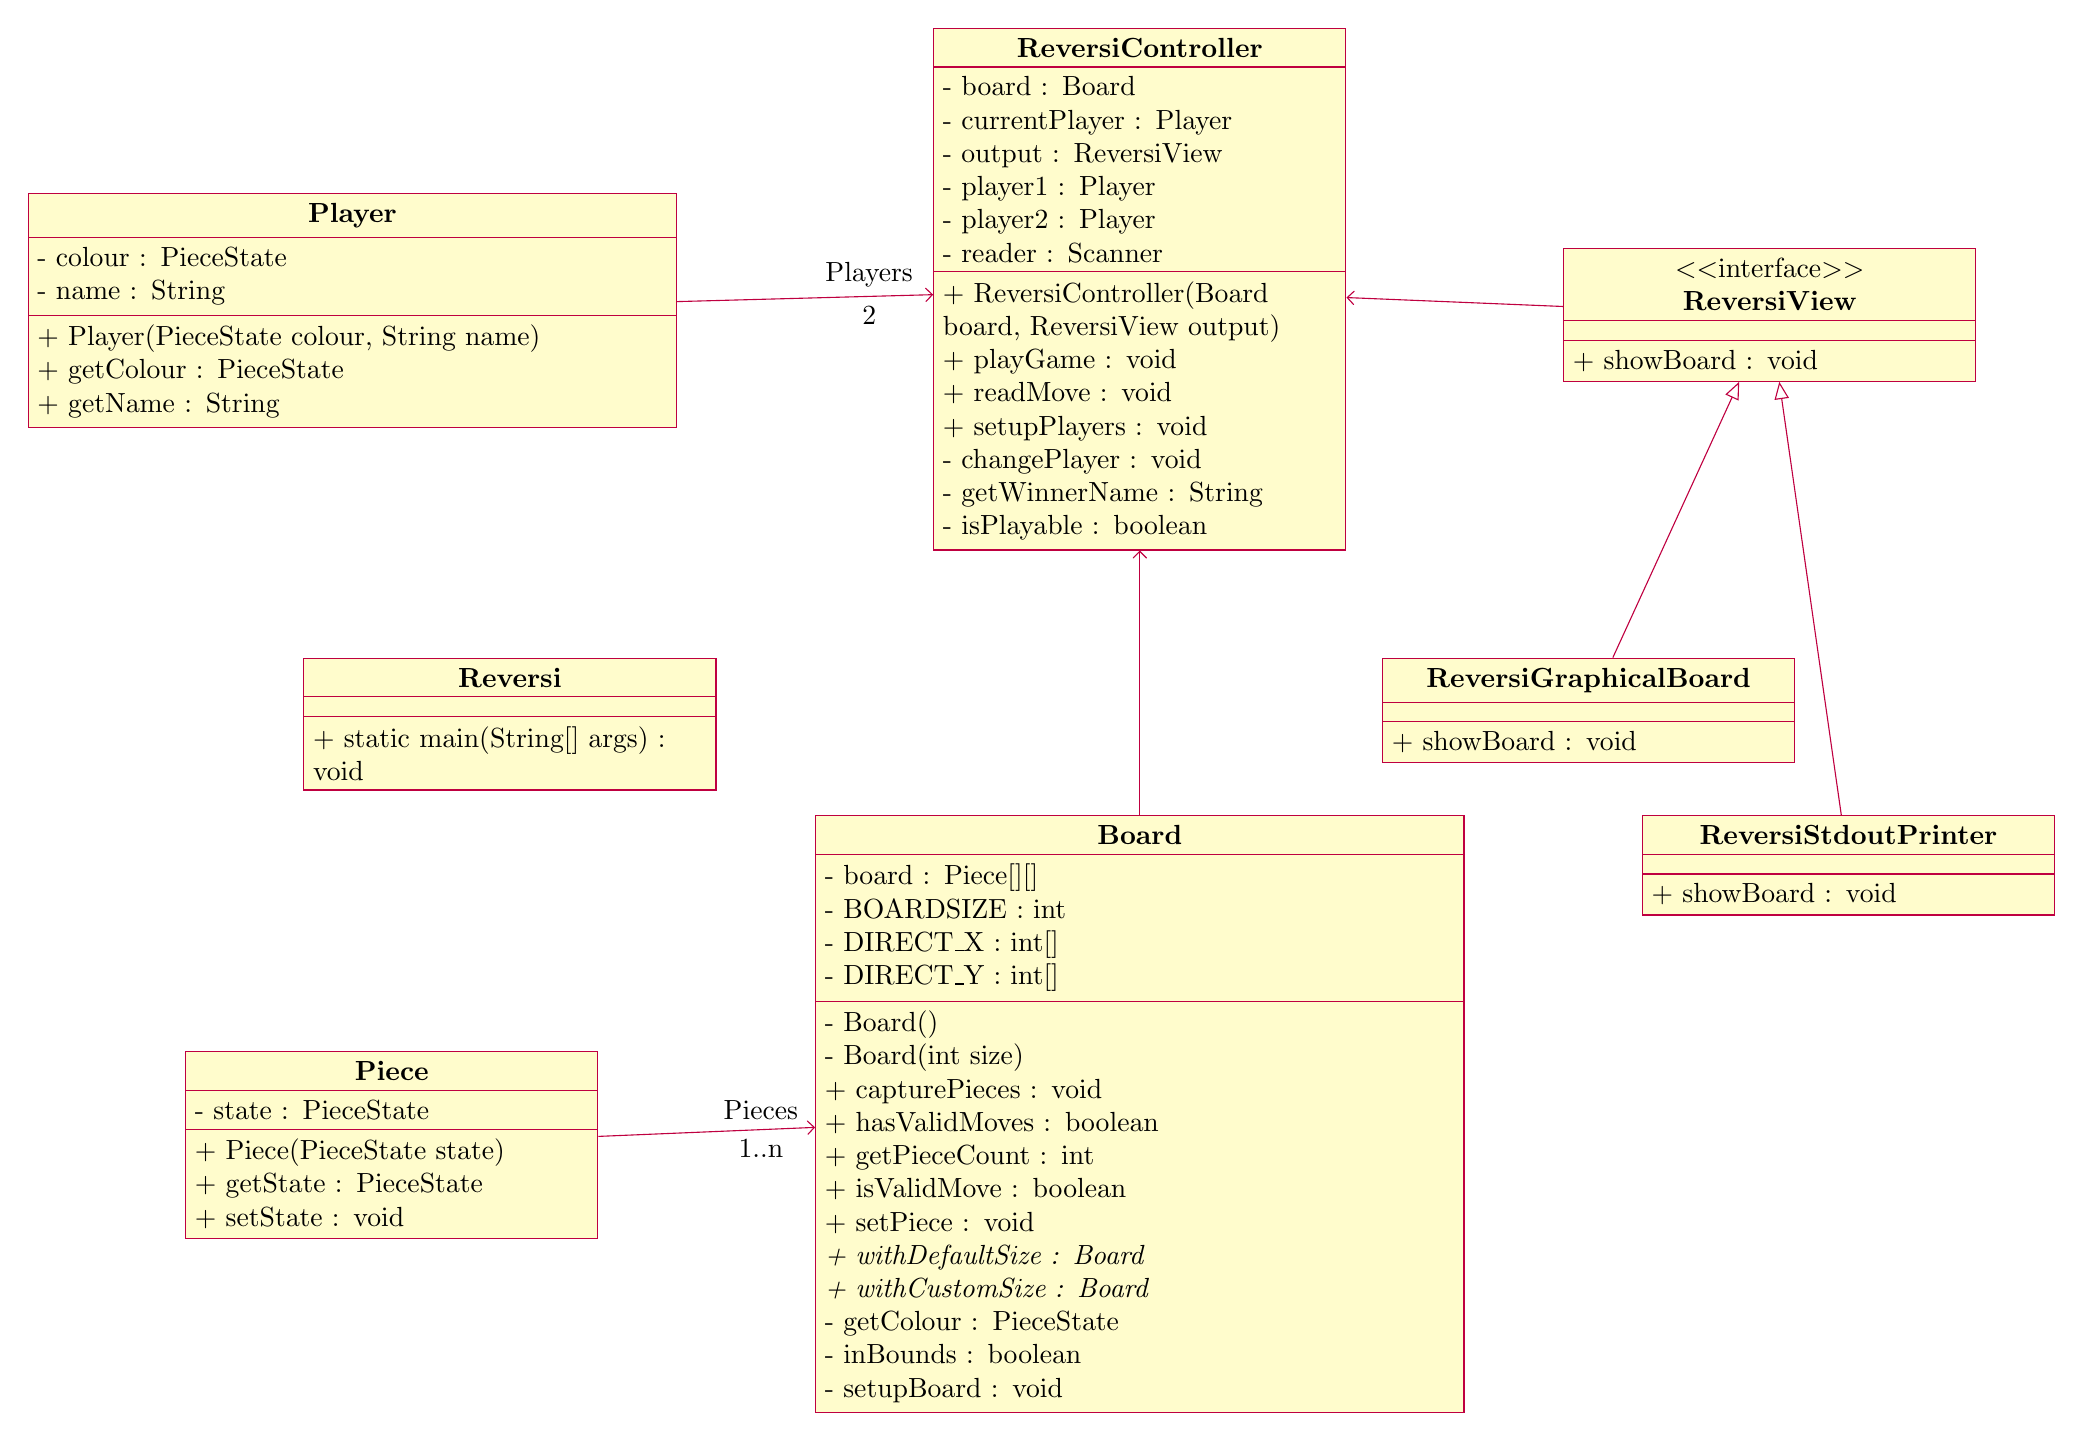
\begin{tikzpicture}
\begin{class}{ReversiController}{12,16} 
\attribute{- board : Board}
\attribute{- currentPlayer : Player}
\attribute{- output : ReversiView}
\attribute{- player1 : Player}
\attribute{- player2 : Player}
\attribute{- reader : Scanner}
\operation{+ ReversiController(Board board, ReversiView output)} 
\operation{+ playGame : void}
\operation{+ readMove : void}
\operation{+ setupPlayers : void}
\operation{- changePlayer : void}
\operation{- getWinnerName : String}
\operation{- isPlayable : boolean}
\end{class}

\begin{class}[text width=8cm]{Board}{12,6}
\attribute{- board : Piece[][]}
\attribute{- BOARDSIZE : int}
\attribute{- DIRECT\_X : int[]}
\attribute{- DIRECT\_Y : int[]}
\operation{- Board()}
\operation{- Board(int size)}
\operation{+ capturePieces : void}
\operation{+ hasValidMoves : boolean}
\operation{+ getPieceCount : int}
\operation{+ isValidMove : boolean}
\operation{+ setPiece : void}
\operation[0]{+ withDefaultSize : Board}
\operation[0]{+ withCustomSize : Board}
\operation{- getColour : PieceState}
\operation{- inBounds : boolean}
\operation{- setupBoard : void}
\end{class}

\begin{interface}{ReversiView}{20,13.2}
\operation{+ showBoard : void}
\end{interface}

\begin{class}{ReversiStdoutPrinter}{21,6}
\inherit{ReversiView}
\operation{+ showBoard : void}
\end{class}

\begin{class}{ReversiGraphicalBoard}{17.7,8}
\inherit{ReversiView}
\operation{+ showBoard : void}
\end{class}

\begin{class}[text width=8cm]{Player}{2, 13.9}
\attribute{- colour : PieceState}
\attribute{- name : String}
\operation{+ Player(PieceState colour, String name)}
\operation{+ getColour : PieceState}
\operation{+ getName : String}
\end{class}

\begin{class}{Piece}{2.5,3}
\attribute{- state : PieceState}
\operation{+ Piece(PieceState state)}
\operation{+ getState : PieceState}
\operation{+ setState : void}
\end{class}

% not sure how to do this
%
% \begin{umlenum}{PieceState}{0,0}
% \attribute{EMPTY}
% \attribute{WHITE}
% \attribute{BLACK}
% \end{umlenum}

\begin{class}{Reversi}{4,8}
\operation{+ static main(String[] args) : void}
\end{class}

\unidirectionalAssociation{Player}{Players}{2}{ReversiController}
\unidirectionalAssociation{Piece}{Pieces}{1..n}{Board}
\unidirectionalAssociation{Board}{}{}{ReversiController}
\unidirectionalAssociation{ReversiView}{}{}{ReversiController}

\end{tikzpicture}
\end{sidewaysfigure}

\subsection*{Reversi}
This class acts as the entry point for the program. The only thing this class does is instantiate the Model, View and Controller, and checks to make sure the command line arguments (if any) are valid. Then it calls the controller to start the game.

\subsection*{Controller}
\subsubsection*{ReversiController}
The controller manages the game. It creates the two players, gives them names and colours, and keeps track of which player can go in the current turn. It starts the game, reading in moves from stdin and converting them to integer input which it then uses to manipulate the model (the part of the model it accesses is the Board class). After each moves it checks if the game is over. If it isn't then it reads the next move from the other player, if it is then it declares the winner.

\subsubsection*{Player}
This simple class keeps track of the player's name and colour. These private fields are encapsulated and getters are provided for them (as is the case throughout the project).

\subsection*{Model}
\subsubsection*{Board}
This class is the basis of the model in the program. It holds the data structure representing the game board itself (in the form of a 2D array of Piece objects), and provides methods to manipulate the data structure: it can get and set the state of pieces in the board, check if a move is valid, check if a Piece of a certain colour can be played anywhere on the board, flip the pieces that should be flipped once a piece has been played, and count the number of pieces of a particular colour on the board.\\
\indent The Board class can be constructed in multiple ways - with a single integer argument which denotes the size of the board, or without any arguments (in which case the default size of 8 is used). We implemented this using the Factory pattern, as originally it was not at all clear what the constructor with the integer did without delving into the class definition. For this Factory pattern we defined two static methods, called \texttt{withDefaultSize()} and \texttt{withCustomSize(int size)}, which insantiate the private contructors \texttt{Board()} and \texttt{Board(int size)} respectively. In both contructors, the board is then set up with the four central pieces filled with alternating tiles (this rule is specific to Othello and not used in Reversi). 

\subsubsection*{Piece}
This class represents a piece that can be placed on the board. It holds a field which represents the colour of the piece (either BLACK, WHITE or EMPTY). The class provides a getter and a setter for this field, which can be used when flipping a piece on the board. 

\subsubsection*{PieceState}
This enumeration is used by the Piece class to store its colour, and also by the Player class, to store which colour each player is playing with. We used the one enum for both to ensure the avoidance of uneccessary code duplication.

\subsection*{Views}
\subsubsection*{ReversiView}
This interface can be implemented by any concrete view of the game, in order to easily plug in to the model and the controller. It has one method, \texttt{showBoard()}, which can be used by a view implementing the interface to print or refresh the board in whichever way it chooses.

\subsubsection*{ReversiStdoutPrinter}
This is our simplest implementation of the ReversiView interface. It prints the board to the console, with row numbers and column letters. It uses dots for empty spaces and W and B for the colours.

\subsubsection*{ReversiGraphicalBoard}
We decided that a good demonstration of the interoperability between our project componants would be to implement another view, which would be very simple to plug in to the already created system. We created a simple graphical representation of the board, using the same symbols as in \texttt{ReversiStdoutPrinter} to keep things consistent. We used the \texttt{javax.swing} and the \texttt{java.awt} packages to implement this view. The window itself is a simple \texttt{JWindow}, with a \texttt{JPanel} for the board, rows and columns. The panels contain multiple \texttt{JLabel}s which show the data from the board, and update when the \texttt{showBoard()} method is called.

\section*{Screenshots}
Here are some screenshots which show our applciation running, and the two different views we created.\\

\noindent
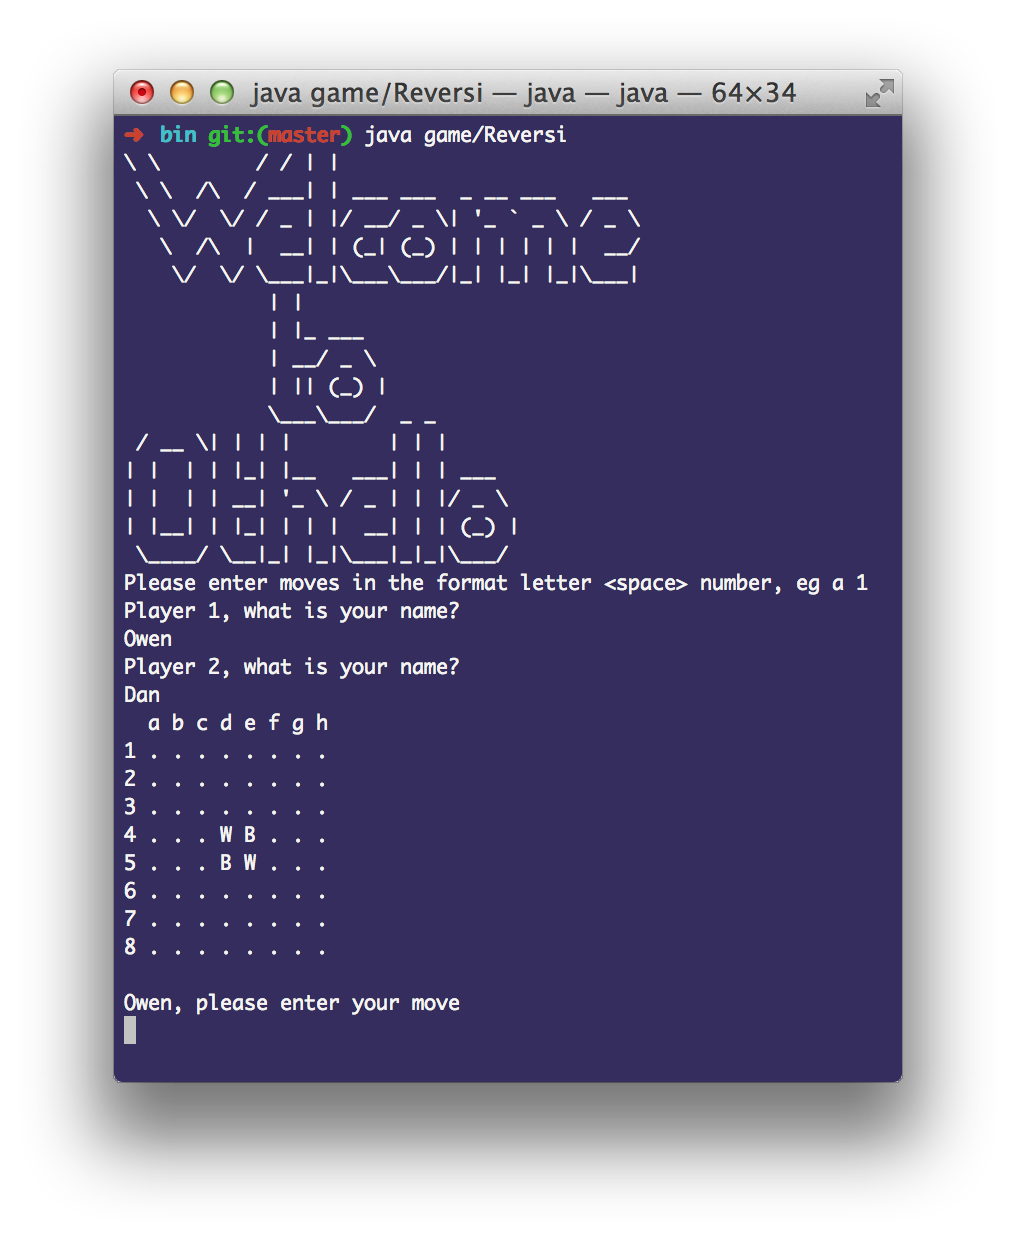
\includegraphics[width=0.5\textwidth]{screenies/gamestart}
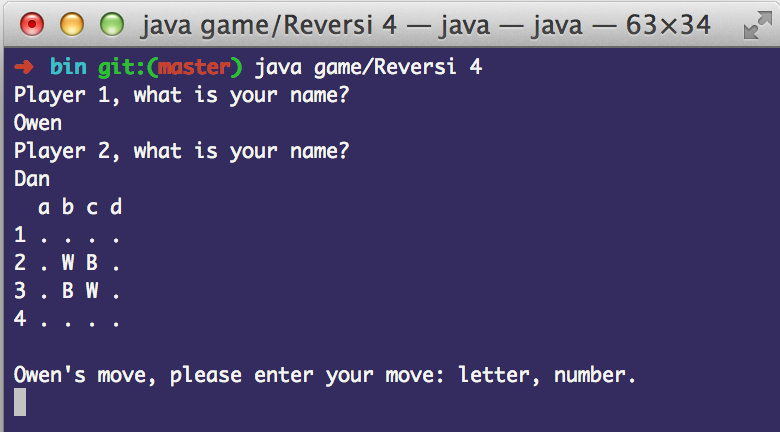
\includegraphics[width=0.5\textwidth]{screenies/startsmall}\\

\noindent The fisrt capture shows the start of a game when using the \texttt{ReversiStdoutView}. The game requests the players' names (using the \texttt{java.util.Scanner} in the controller), and prints the inital game board. The second capture demonstrates how a game is started with a custom board size - the \texttt{Reversi} class detects that there is a command line argument and invokes a different factory method in the \texttt{Board} class which constructs the board obect with a custom board size.

\noindent
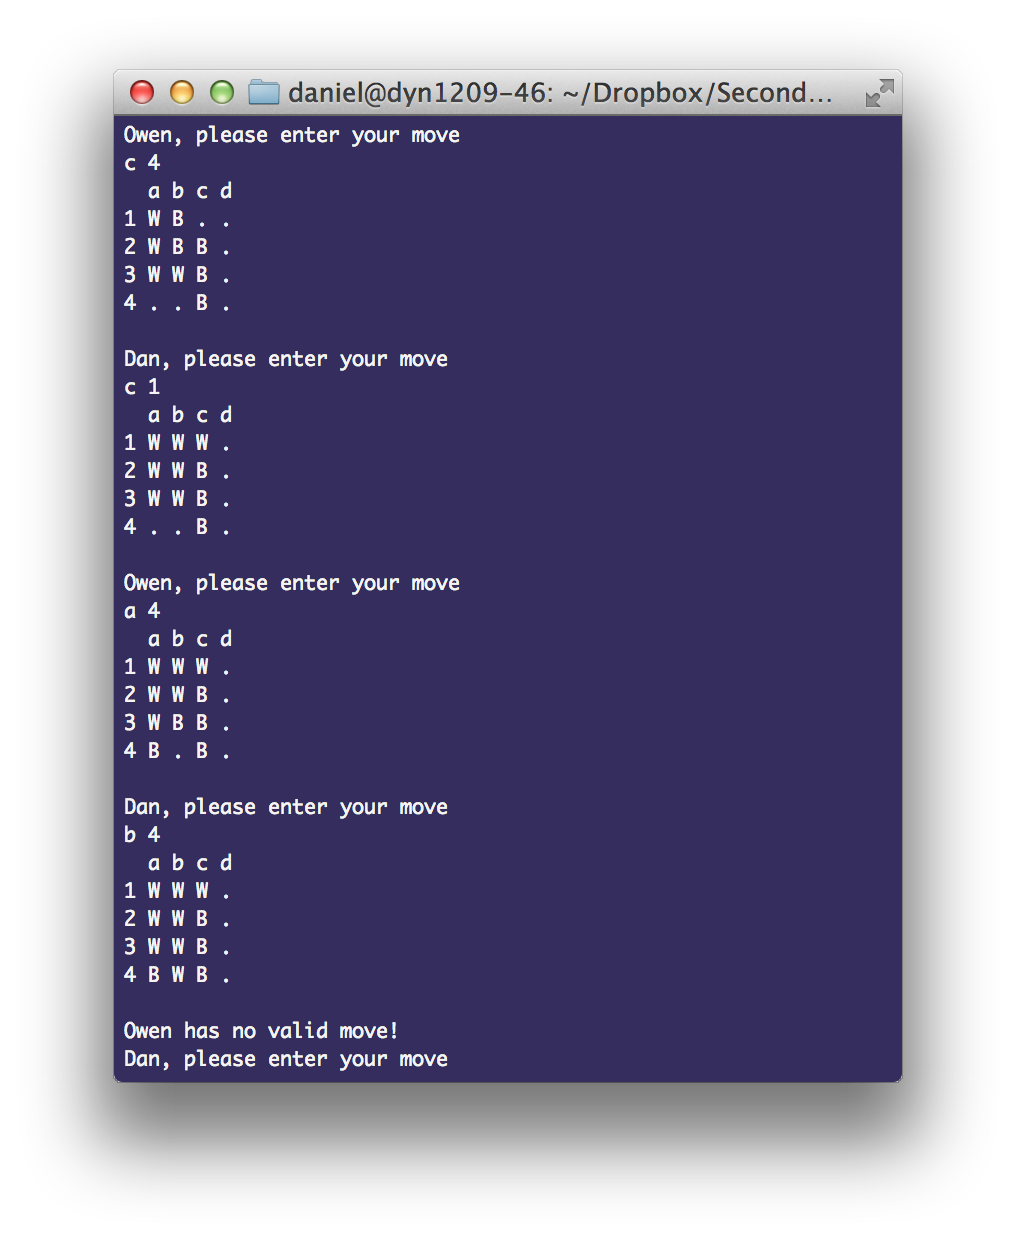
\includegraphics[width=0.5\textwidth]{screenies/invalidsmall}
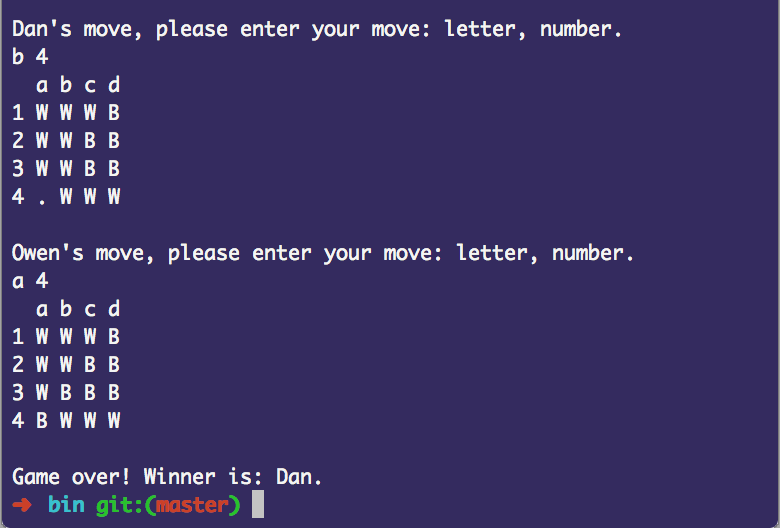
\includegraphics[width=0.5\textwidth]{screenies/winning}\\

\noindent The left-hand capture shows the behaviour of the program when a player can't make any move - the game passes the current move to Dan as Owen cannot legally play anywhere. The right-hand capture demonstrates the game-over behaviour. When no more moves are possible for either player, the controller compares the number of pieces of each colour and declares the winner.\\

\noindent
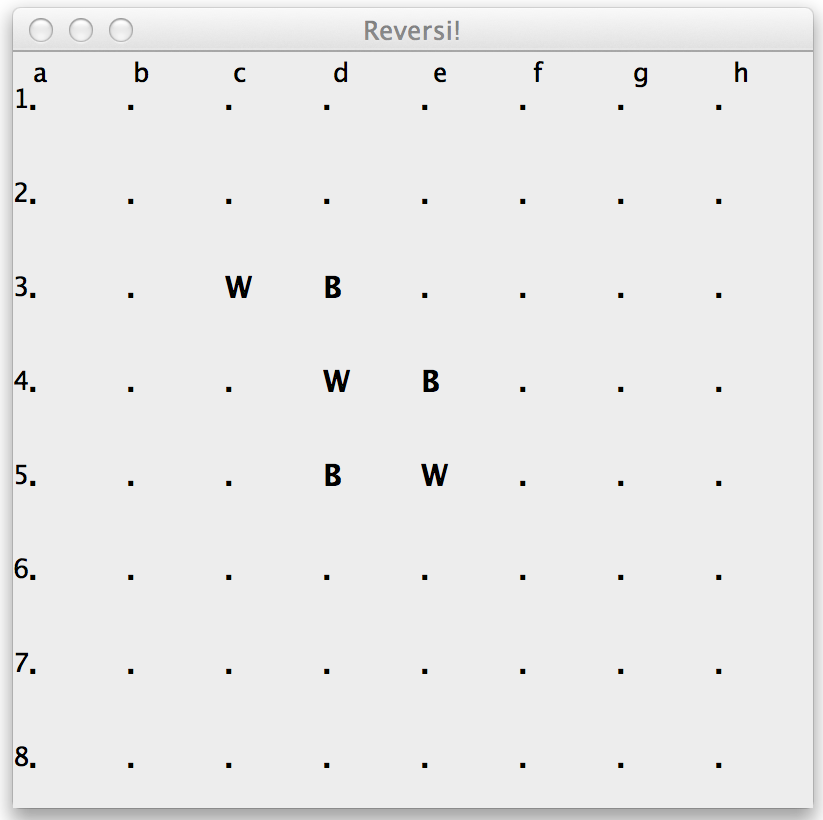
\includegraphics[width=0.5\textwidth]{screenies/graphical}\\

\noindent The final capture shows the (very simple) graphical view we created, demonstrating how we reduced coupling between the view and the model.

\section*{Design Decisions}
In this section we will outline a few design decisions that we made throughout the course of the project.

\begin{itemize}
\item We decided it was not worth using the singleton pattern for the board class. Because we would only ever make one \texttt{Board} object which would be passed to the controller and the view, we decided it was overkill to force the user to only ever have one board.

\item We agreed that it wasn't worth 
\end{itemize}

\end{document}
